\chapter{Fully homomorphic encryption: Construction}\label{chapfhetwo}

In the last lecture we defined fully homomorphic encryption, and showed
the ``bootstrapping theorem'' that transforms a partially homomorphic
encryption scheme into a fully homomorphic encryption, as long as the
original scheme can homomorphically evaluate its own decryption circuit.
In this lecture we will show an encryption scheme (due to Gentry, Sahai
and Waters, henceforth GSW) meeting the latter property. That is, this
lecture is devoted to proving\footnote{This theorem as stated was proven
  by Brakerski and Vaikuntanathan (ITCS 2014) building a line of work
  initiated by Gentry's original STOC 2009 work. We will actually prove
  a weaker version of this theorem, due to Brakerski and Vaikuntanathan
  (FOCS 2011), which assumes a quantitative strengthening of LWE.
  However, we will not follow the proof of Brakerski and Vaikuntanathan
  but rather a scheme of Gentry, Sahai and Waters (CRYPTO 2013). Also
  note that, as noted in the previous lecture, all of these results
  require the extra assumption of \emph{circular security} on top of LWE
  to achieve a non-leveled fully homomorphic encryption scheme.} the
following theorem:

\hypertarget{LWEFHEthm}{}
\begin{theorem}[FHE from LWE] \label[theorem]{LWEFHEthm}

Assuming the LWE conjecture, there exists a partially homomorphic public
key encryption \((G,E,D,\ensuremath{\mathit{EVAL}})\) that fits the
conditions of the bootstrapping theorem (\cref{bootstrapthm}). That is,
for every two ciphertexts \(c\) and \(c'\), the function
\(d \mapsto D_d(c)\; \ensuremath{\mathit{NAND}}\; D_d(c')\) can be
homomorphically evaluated by \(\ensuremath{\mathit{EVAL}}\).

\end{theorem}

Before the detailed description and analysis, let us first outline our
strategy. Something of essential importance is the following.

::: \# \{.definition title=``Noisy Homomorphic Encryption''
\#NoisyHEdef\} Suppose that \((G,E,D)\) is a CPA secure public key
scheme and that \(\eta\) is a measure which maps any ciphertext \(c\) to
its ``noise'' \(\eta(c)\in [0, \infty).\) Denote
\[\mathcal{C}_b^\theta=\{c:D_b(c)=b,\eta(c)\leq\theta \}.\]
\((G,E,D,\ensuremath{\mathit{NAND}})\) is called a \emph{noisy
homomorphic encryption scheme} if the followings holds for some
\(q=q(n)\):

\begin{itemize}
\item
  \(E_e(b)\in \mathcal{C}_b^{\sqrt{q}}\) for any plaintext \(b\).
\item
  If \(c\in\mathcal{C}_b^\eta\) with \(\eta\leq q/4\), then
  \(D_e(c)=b\).
\item
  For any \(c\in\mathcal{C}_b^\eta\) and
  \(c'\in\mathcal{C}_{b'}^{\eta'}\), it holds that
  \[\ensuremath{\mathit{ENAND}}(c,c')\in\mathcal{C}_{b\overline{\wedge}b'}^{n^3\cdot \max\{\eta,\eta'\}}\]
  as long as \(n^3\cdot \max\{\eta,\eta'\}<q/4\). :::
\end{itemize}

The noisy homomorphic encryption actually states that if \(C\) and
\(C'\) encrypt \(b\) and \(b'\) up to error \(\eta\) and \(\eta'\),
respectively, then \(\ensuremath{\mathit{ENAND}}(c,c')\) encrypts
\(\ensuremath{\mathit{NAND}}(b,b')\) up to some error which can be
controlled by \(\eta,\eta'\). The coefficient \(n^3\) is not essential
here; we just need the order \(poly(n)\). This property allows us to
perform the \(\ensuremath{\mathit{ENAND}}\) operator repeatly as long as
we can guarantee the accumulated error is smaller than \(q/4\), which
means that the decryption can be done correctly. The next theorem tells
us with what depth, a circuit that can be computed homomorphically.

\hypertarget{Depththm}{}
\begin{theorem} \label[theorem]{Depththm}

If there exists a noisy homomorphic encryption scheme with
\(q=2^{\sqrt{n}}\), then the it can be extended to a homomorphic
encryption scheme for any circuit with depth smaller than
\(polylog(n)\).

\end{theorem}

\begin{proof} \label[proof]{For-any-function-fmrightarrow-}

For any function \(f:\{0,1\}^m\rightarrow \{0,1\}\) which can be
described by a circuit with depth \(\ell\), we can compute
\(\ensuremath{\mathit{EVAL}}(f,E_e(x_1),\cdots,E_e(x_m))\) with error up
to \(\sqrt(q)(n^3)^\ell\). (The initial error for \(E_e(x_i)\) is
smaller than \(\sqrt{n}\) and the error will be accumulated with rate up
to \(n^3\).) Thus, to guarantee that
\(\ensuremath{\mathit{EVAL}}(f,E_e(x_1),\cdots,E_e(x_m))\) can be
decrypted to \(f(x_1,\cdots,x_m)\) correctly, we only need
\(\sqrt(q)(n^3)^\ell\ll q\), i.e.,
\(n^{3\ell}\ll \sqrt{q}=2^{\sqrt{n}/2}\). This is equalvent to
\(3\ell\log(n)\ell \sqrt{n}/2\), which can be guaranteed when
\(\ell =n^{o(1)}\) or \(\ell=polylog(n)\).

\end{proof}

With \cref{Depththm}, the rest is to verify that the function
\(d \mapsto D_d(c)\; \ensuremath{\mathit{NAND}}\; D_d(c')\) can be
computed by a circuit with depth being \(polylog(n)\). And then we can
obtain a fully homomorphic encryption scheme. We will head into some
details show how to construct things we want in the rest of this
chapter. The most technical and interesting part would be how to
upperbound the noise/error.

\section{Prelude: from vectors to
matrices}\label{Prelude-from-vectors-to-matric}

In the linear homomorphic scheme we saw in the last lecture, every
ciphertext was a vector \(c\in\Z_q^n\) such that \(\langle c,s \rangle\)
equals (up to scaling by \(\floor{\tfrac{q}{2}}\)) the plaintext bit. We
saw that adding two ciphertexts modulo \(q\) corresponded to XOR'ing
(i.e., adding modulo \(2\)) the corresponding two plaintexts. That is,
if we define \(c \oplus c'\) as \(c+c' \pmod{q}\) then performing the
\(\oplus\) operation on the ciphertexts corresponds to adding modulo
\(2\) the plaintexts.

However, to get to a fully, or even partially, homomorphic scheme, we
need to find a way to perform the NAND operation on the two plaintexts.
The challenge is that it seems that to do that we need to find a way to
evaluate \emph{multiplications}: find a way to define some operation
\(\otimes\) on ciphertexts that corresponds to multiplying the
plaintexts. Alas, a priori, there doesn't seem to be a natural way to
\emph{multiply} two vectors.

The GSW approach to handle this is to move from vectors to
\emph{matrices}. As usual, it is instructive to first consider the
cryptographer's dream world where Gaussian elimination doesn't exist. In
this case, the GSW ciphertext encrypting \(b\in\{0,1\}\) would be an
\(n\times n\) matrix \(C\) over \(\Z_q\) such that \(Cs = bs\) where
\(s\in\Z_q^n\) is the secret key. That is, the encryption of a bit \(b\)
is a matrix \(C\) such that the secret key is an \emph{eigenvector}
(modulo \(q\)) of \(C\) with corresponding eigenvalue \(b\). (We defer
discussion of how the encrypting party generates such a ciphertext,
since this is in any case only a ``dream'' toy example.)

\begin{pause} \label[pause]{You-should-make-sure-you-under}

You should make sure you understand the \emph{types} of all the
identifiers we refer to. In particular, above \(C\) is an \(n\times n\)
\emph{matrix} with entries in \(\Z_q\), \(s\) is a \emph{vector} in
\(\Z_q^n\), and \(b\) is a \emph{scalar} (i.e., just a number) in
\(\{0,1\}\). See \cref{naivegswfig} for a visual representation of the
ciphertexts in this ``naive'' encryption scheme. Keeping track of the
dimensions of all objects will become only more important in the rest of
this lecture.

\end{pause}

\begin{marginfigure}
\centering
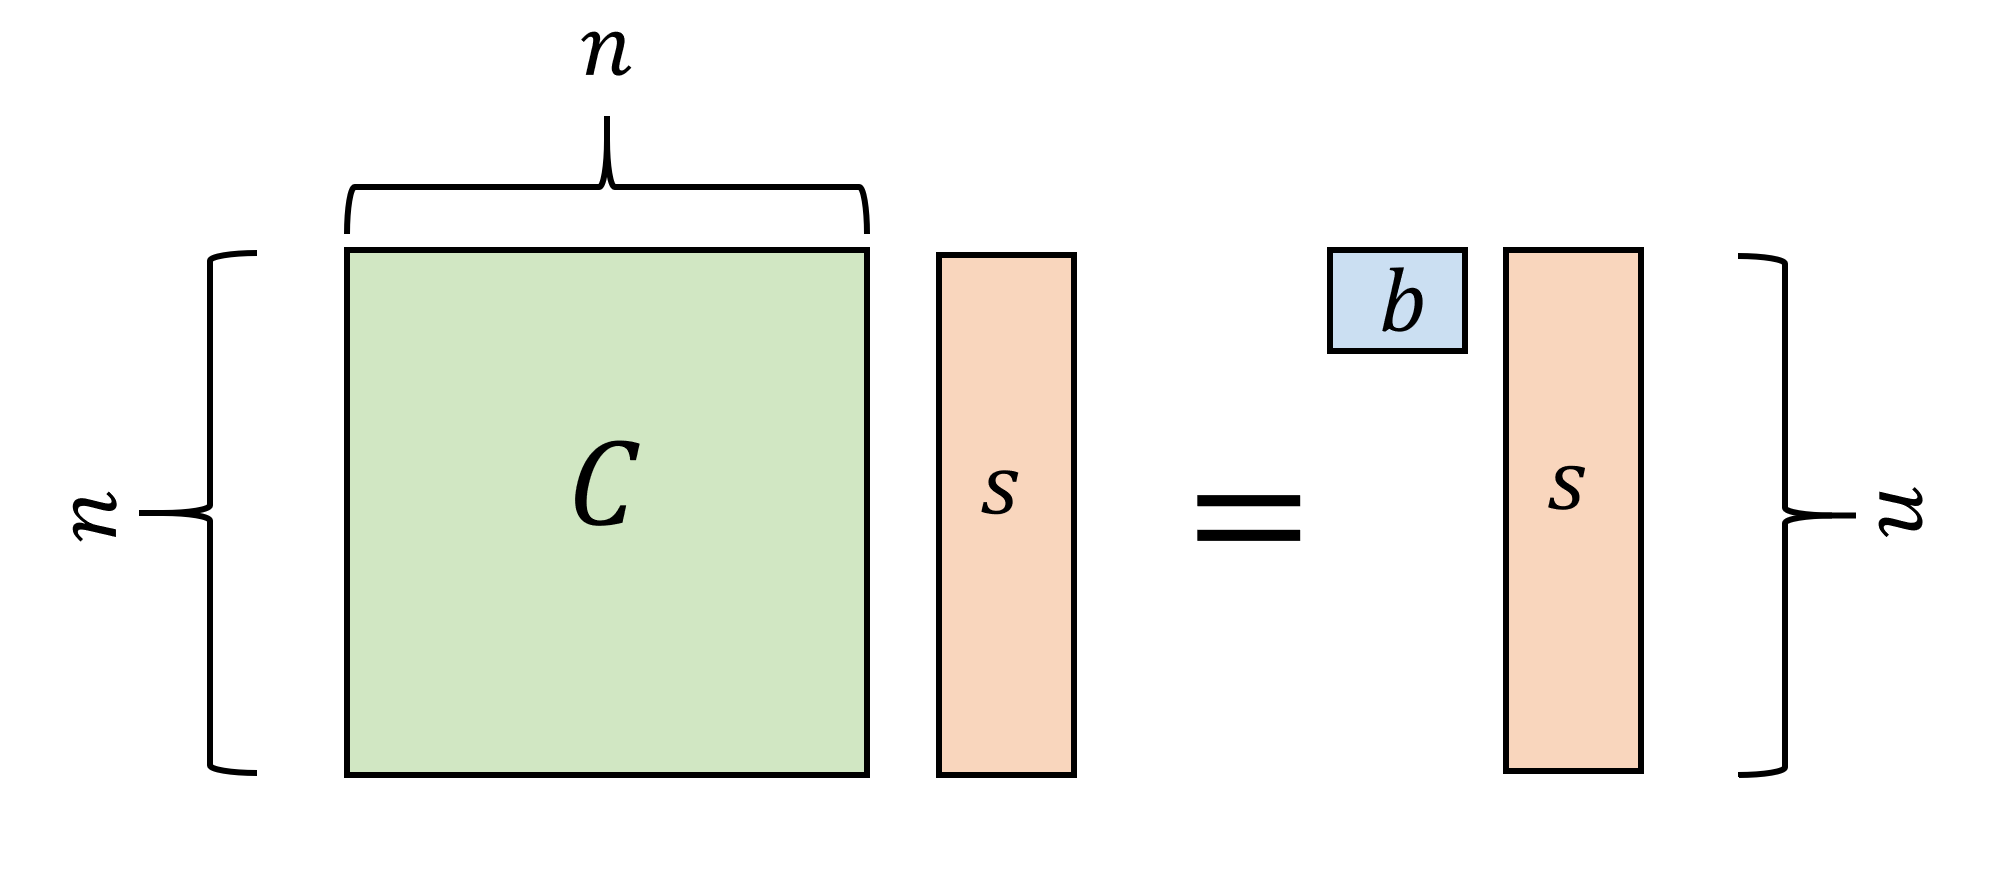
\includegraphics[width=\linewidth, height=1.5in, keepaspectratio]{../figure/naivegsw.png}
\caption{In the ``naive'' version of the GSW encryption, to encrypt a
bit \(b\) we output an \(n\times n\) matrix \(C\) such that \(Cs=bs\)
where \(s \in \Z_q^n\) is the secret key. In this scheme we can
transform encryptions \(C,C'\) of \(b,b'\) respectively to an encryption
\(C''\) of \(\ensuremath{\mathit{NAND}}(b,b')\) by letting
\(C'' = I-CC'\).}
\label{naivegswfig}
\end{marginfigure}

Given \(C\) and \(s\) we can recover \(b\) by just checking if \(Cs=s\)
or \(Cs=0^n\). The scheme allows homomorphic evaluation of both addition
(modulo \(q\)) and multiplication, since if \(Cs = bs\) and \(C's=b's\)
then we can define \(C \oplus C' = C + C'\) (where on the righthand
side, addition is simply done in \(\Z_q\)) and
\(C\otimes C' = \ensuremath{\mathit{CC}}'\) (where again this refers to
matrix multiplication in \(\Z_q\)).

Indeed, one can verify that both addition and multiplication succeed
since \[(C+C')s = (b+b')s\] and
\[\ensuremath{\mathit{CC}}'s = C(b's) = bb's\] where all these
equalities are in \(\Z_q\).

Addition modulo \(q\) is not the same as XOR, but given these
multiplication and addition operations, we can implement the NAND
operation as well. Specifically, for every \(b,b' \in \{0,1\}\),
\(b \; \ensuremath{\mathit{NAND}} \; b' = 1-bb'\). Hence we can take a
ciphertext \(C\) encrypting \(b\) and a ciphertext \(C'\) encrypting
\(b'\) and transform these two ciphertexts to the ciphertext
\(C''=(I-CC')\) that encrypts \(b\; \ensuremath{\mathit{NAND}} \; b'\)
(where \(I\) is the identity matrix). Thus in a world without Gaussian
elimination it is not hard to get a fully homomorphic encryption.

\hypertarget{privkeyfhe}{}
\begin{remark}[Private key FHE] \label[remark]{privkeyfhe}

We have not shown how to \emph{generate} a ciphertext without knowledge
of \(s\), and hence strictly speaking we only showed in this world how
to get a \emph{private key} fully homomorphic encryption. Our ``real
world'' scheme will be a full fledged \emph{public key} FHE. However we
note that private key homomorphic encryption is already very interesting
and in fact sufficient for many of the ``cloud computing'' applications.
Moreover, \href{http://eccc.hpi-web.de/report/2010/146/}{Rothblum} gave
a generic transformation from a \emph{private key} homomorphic
encryption to a \emph{public key} homomorphic encryption.

\end{remark}

\section{Real world partially homomorphic
encryption}\label{Real-world-partially-homomorph}

We now discuss how we can obtain an encryption in the real world where,
as much as we'd like to ignore it, there are people who walk among us
(not to mention some computer programs) that actually know how to invert
matrices. As usual, the idea is to ``fool Gaussian elimination with
noise'' but we will see that we have to be much more careful about
``noise management'', otherwise even for the party holding the secret
key the noise will overwhelm the signal.\footnote{For this reason, Craig
  Gentry called his highly recommended survey on fully homomorphic
  encryption and other advanced constructions
  \href{https://eprint.iacr.org/2014/610}{computing on the edge of
  chaos}.}

The main idea is that we can expect the following problem to be hard for
a random secret \(s\in\Z_q^n\): distinguish between samples of random
matrices \(C\) and matrices where \(Cs = bs + e\) for some
\(b\in\{0,1\}\) and ``short'' \(e\) satisfying \(|e_i| \leq \sqrt{q}\)
for all \(i\). This yields a natural candidate for an encryption scheme
where we encrypt \(b\) by a matrix \(C\) satisfying \(Cs = bs + e\)
where \(e\) is a ``short'' vector.\footnote{We deliberately leave some
  flexibility in the definition of ``short''. While initially ``short''
  might mean that \(|e_i|<\sqrt{q}\) for every \(i\), decryption will
  succeed as long as long as \(|e_i|\) is, say, at most \(q/100\).}

We can now try to check what adding and multiplying two matrices does to
the noise. If \(Cs = bs+e\) and \(C's=b's+e'\) then
\[(C+C')s = (b+b')s+(e+e') \label{eqhomadd}\] and
\[\ensuremath{\mathit{CC}}'s = C(b's+e')+e =bb's+ (b'e+Ce')\;. \label{eqhommult} \]

\begin{pause} \label[pause]{I-recommend-you-pause-here-and}

I recommend you pause here and check for yourself whether it will be the
case that if \(C+C'\) encrypts \(b+b'\) and
\(\ensuremath{\mathit{CC}}'\) encrypts \(bb'\) up to small noise or not.

\end{pause}

We would have loved to say that we can define as above
\(C\oplus C' = C+C' (\mod\; q)\) and
\(C\otimes C' = \ensuremath{\mathit{CC}}' (\mod \; q)\). For this we
would need that \((C+C')s\) equals \((b+b')s\) plus a ``short'' vector
and \(\ensuremath{\mathit{CC}}'s\) equals \(bb's\) plus a ``short''
vector. The former statement indeed holds. Looking at \eqref{eqhommult}
we see that \((C+C')s\) equals \((b+b')s\) up to the ``noise'' vector
\(e+e'\), and if \(e,e'\) are ``short'' then \(e+e'\) is not too long
either. That is, if \(|e_i|<\delta q\) and \(|e'_i|<\delta q\) for every
\(i\) then \(|e_i+e'_i|<2\delta q\). So we can at least handle a
significant number of additions before the noise gets out of hand.

However, if we consider \eqref{eqhommult}, we see that
\(\ensuremath{\mathit{CC}}'\) will be equal to \(bb's\) plus the ``noise
vector'' \(b'e + Ce'\). The first component \(b'e\) of this noise vector
is ``short'' (after all \(b\in \{0,1\}\) and \(e\) is ``short'').
However, the second component \(Ce'\) could be a very large vector.
Indeed, since \(C\) looks like a random matrix in \(\Z_q\), no matter
how small the entries of \(e'\), many of the entries of \(Ce'\) are
quite likely to be of magnitude at least, say, \(q/2\) and so
multiplying \(e'\) by \(C\) takes us ``beyond the edge of chaos''.

\section{Noise management via
encoding}\label{Noise-management-via-encoding}

The problem we had above is that the entries of \(C\) are elements in
\(\Z_q\) that can be very large, while we would have loved them to be
small numbers such as \(0\) or \(1\). At this point one could say

\begin{quote}
\emph{``If only there was some way to encode numbers between \(0\) and
\(q-1\) using only \(0\)'s and \(1\)'s''}
\end{quote}

If you think about it hard enough, it turns out that there is something
known as the ``binary basis'' that allows us to encode a number
\(x\in\Z_q\) as a vector \(\hat{x}\in\{0,1\}^{\log q}\).\footnote{If we
  were being pedantic the length of the vector (and other constant
  below) should be the integer \(\ceil{\log q}\) but I omit the ceiling
  symbols for simplicity of notation.} What's even more surprising is
that this seemingly trivial trick turns out to be immensely useful. We
will define the \emph{binary encoding} of a vector or matrix \(x\) over
\(\Z_q\) by \(\hat{x}\). That is, \(\hat{x}\) is obtained by replacing
every coordinate \(x_i\) with \(\log q\) coordinates
\(x_{i,0},\ldots,x_{i,\log q-1}\) such that

\[x_i = \sum_{j=0}^{\log q-1}2^j x_{i,j} \;. \label{eqbinaryencoding}\]

Specifically, if \(s\in \Z_q^n\), then we denote by \(\hat{s}\) the
\(n\log q\)-dimensional vector with entries in \(\{0,1\}\), such that
each \(\log q\)-sized block of \(\hat{s}\) encodes a coordinate of
\(s\). Similarly, if \(C\) is an \(m\times n\) matrix, then we denote by
\(\hat{C}\) the \(m\times n\log q\) matrix with entries in \(\{0,1\}\)
that corresponds to encoding every \(n\)-dimensional row of \(C\) by an
\(n\log q\)-dimensional row where each \(\log q\)-sized block
corresponds to a single entry. (We still think of the entries of these
vectors and matrices as elements of \(\Z_q\) and so all calculations are
still done modulo \(q\).)

While encoding in the binary basis is not a linear operation, the
\emph{decoding} operation is linear as one can see in
\eqref{eqbinaryencoding}. We let \(Q\) be the \(n \times (n\log q)\)
``decoding'' matrix that maps an encoding vector \(\hat{s}\) back to the
original vector \(s\). Specifically, every row of \(Q\) is composed of
\(n\) blocks each of \(\log q\) size, where the \(i\)-th row has only
the \(i\)-th block nonzero, and equal to the values
\((1,2,4,\ldots,2^{\log q-1})\). It's a good exercise to verify that for
every vector \(s\in \Z_q^n\) and matrix \(C\in \Z_q^{n\times n}\),
\(Q\hat{s}=s\) and \(\hat{C}Q^\top =C\). (See \cref{encodevecfig} amd
\cref{encodematrixfig}.)

\begin{marginfigure}
\centering
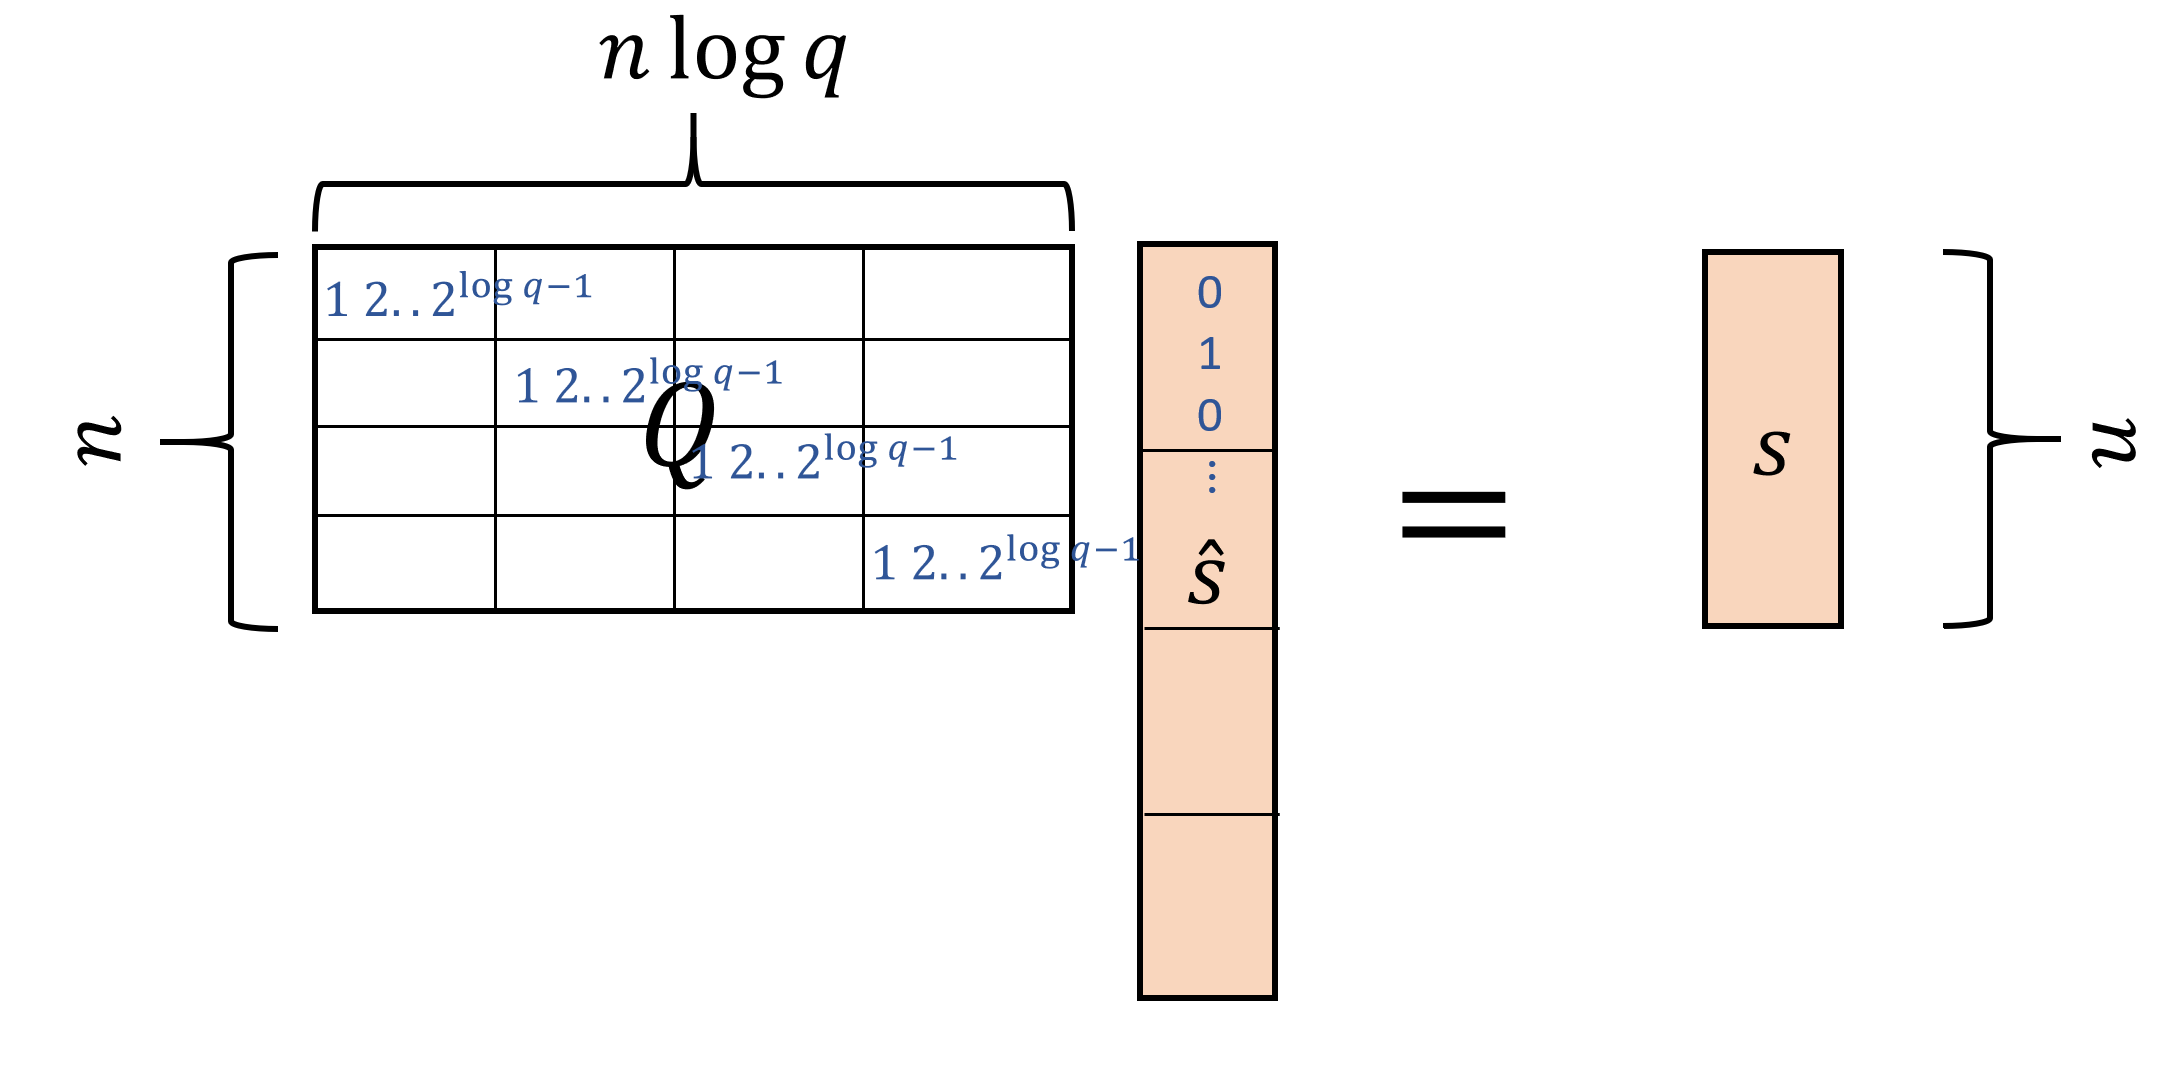
\includegraphics[width=\linewidth, height=1.5in, keepaspectratio]{../figure/encodevec.png}
\caption{We can encode a vector \(s\in \Z_q^n\) as a vector
\(\hat{s} \in \Z_q^{n\log q}\) that has only entries in \(\{0,1\}\) by
using the binary encoding, replacing every coordinate of \(s\) with a
\(\log q\)-sized block in \(\hat{s}\). The decoding operation is
\emph{linear} and so we can write \(s=Q\hat{s}\) for a specific (simple)
\(n \times (n\log q)\) matrix \(Q\).}
\label{encodevecfig}
\end{marginfigure}

\begin{marginfigure}
\centering
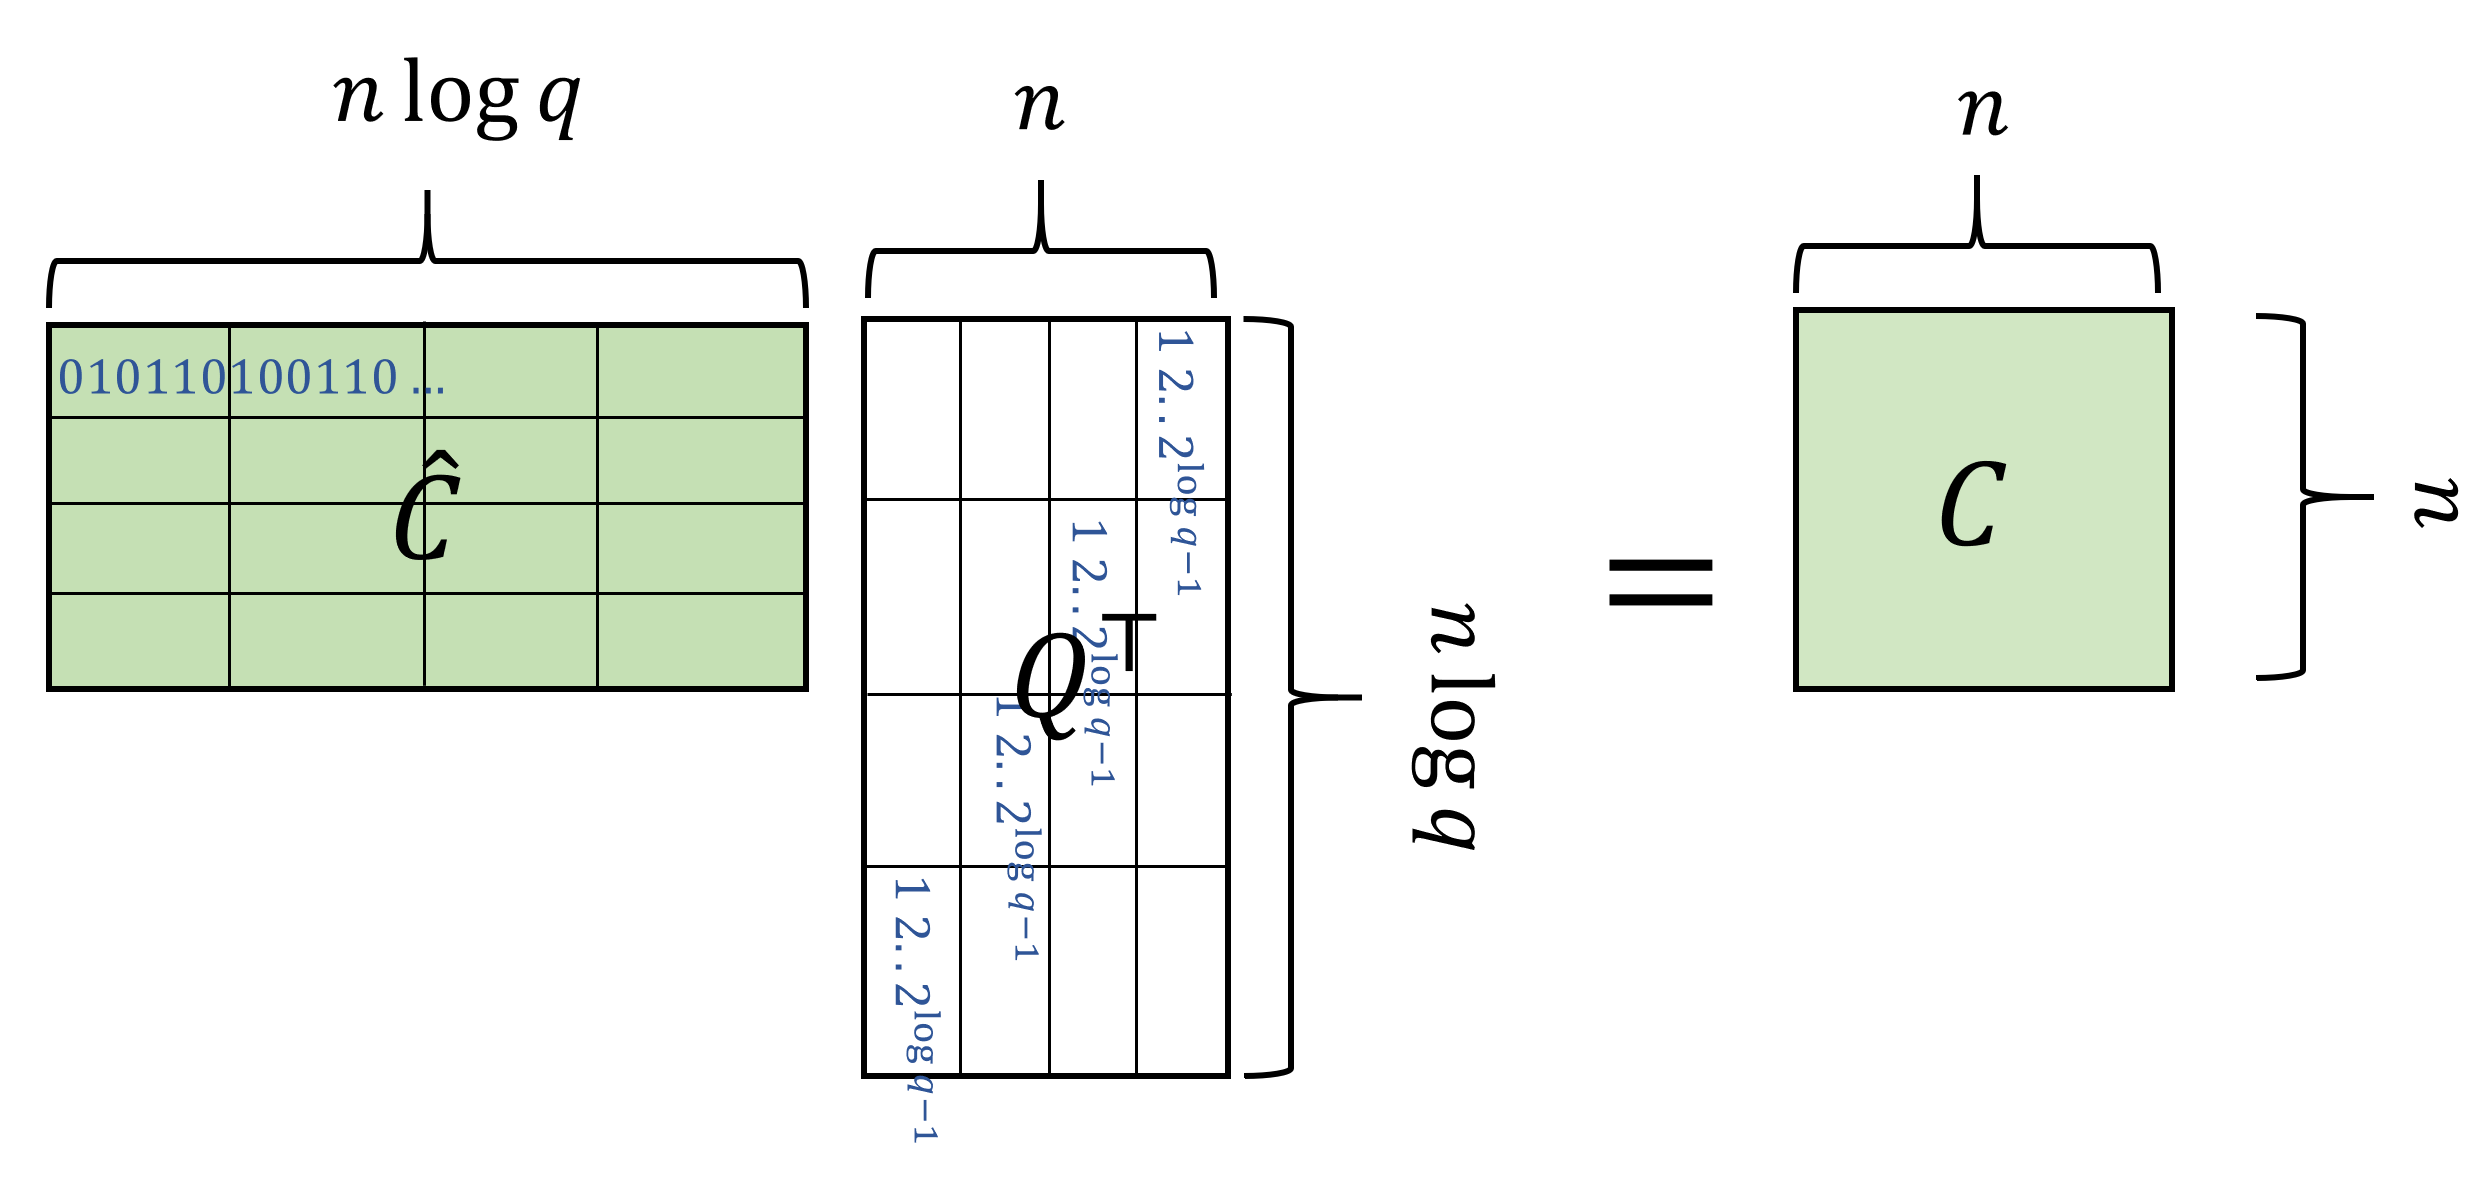
\includegraphics[width=\linewidth, height=1.5in, keepaspectratio]{../figure/encodematrix.png}
\caption{We can encode an \(n\times n\) matrix \(C\) over \(\Z_q\) by an
\(n\times (n \log q)\) matrix \(\hat{C}\) using the binary basis. We
have the equation \(C=\hat{C}Q^\top\) where \(Q\) is the same matrix we
use to decode a vector.}
\label{encodematrixfig}
\end{marginfigure}

In our final scheme the ciphertext encrypting \(b\) will be an
\((n\log q)\times (n\log q)\) matrix \(C\) with small coefficients such
that \(Cv =bv + e\) for a ``short'' \(e \in \Z_q^{n\log q}\) and
\(v=Q^\top s\) for \(s\in\Z_q^n\). Now given ciphertexts \(C,C'\) that
encrypt \(b,b'\) respectively, we will define
\(C \oplus C' = C + C' \pmod{q}\) and
\(C \otimes C' = \widehat{(\ensuremath{\mathit{CQ}}^\top)}C'\).

Since we have \(Cv = bv + e\) and \(C'v = b'v + e'\) we get that
\[(C\oplus C')v = (C+C')v = (b+b')v + (e+e') \label{eqfheaddfinal}\] and
\[(C\otimes C')v = \widehat{(\ensuremath{\mathit{CQ}}^\top)}C'v = \widehat{(\ensuremath{\mathit{CQ}}^\top)}(b'v+e') \;. \label{fhemultfinaleqfirst}\]

But since \(v=Q^\top s\) and \(\hat{A}Q^\top = A\) for every matrix
\(A\), the righthand side of \eqref{fhemultfinaleqfirst} equals

\[\widehat{(\ensuremath{\mathit{CQ}}^\top)}(b'Q^\top s+e')=b'C Q^\top s+\widehat{(\ensuremath{\mathit{CQ}}^\top)}e' = b'Cv + \widehat{(\ensuremath{\mathit{CQ}}^\top)}e' \label{fhemultfinaleqsec}\]

but since \(\widehat{B}\) is a matrix with small coefficients for every
\(B\) and \(e'\) is short, the righthand side of
\eqref{fhemultfinaleqsec} equals \(b'Cv\) up to a short vector, and
since \(Cv=bv+e\) and \(b'e\) is short, we get that \((C\otimes C')v\)
equals \(b'bv\) plus a short vector as desired.

If we keep track of the parameters in the above analysis, we can see
that

\[C \overline{\wedge} C' = (I - C \otimes C')\]

then if \(C\) encrypts \(b\) and \(C'\) encrypts \(b'\) with noise
vectors \(e,e'\) satisfying \(\max |e_i| \leq \mu\) and
\(\max |e'_i| \leq \mu'\) then \(C \overline{\wedge} C'\) encrypts
\(b \; \ensuremath{\mathit{NAND}}\; b'\) up to a vector of maximum
magnitude at most \(O(\mu + n\log q \mu')\), which is definitely smaller
than \(n^3\cdot \max\{\eta,\eta,\}\) for \(q=2^{\sqrt{n}}\).

\section{Putting it all together}\label{Putting-it-all-together}

We now describe the full scheme. We are going to use a quantitatively
stronger version of LWE. Namely, the \(q(n)\)-dLWE assumption for
\(q(n)=2^{\sqrt{n}}\). It is not hard to show that we can relax our
assumption to \(q(n)\)-LWE \(q(n)=2^{polylog(n)}\) and Brakerski and
Vaikuntanathan showed how to relax the assumption to standard
(i.e.~\(q(n)=poly(n)\)) LWE though we will not present this here.

\begin{quote}
\textbf{FHEENC:}

\begin{itemize}
\item
  \textbf{Key generation:} As in the scheme of last lecture the secret
  key is \(s\in\Z_s^n\) and the public key is a generator \(G_s\) such
  that samples from \(G_s(1^n)\) are indistinguishable from independent
  random samples from \(\Z_q^n\) but if \(c\) is output by \(G_s\) then
  \(|\langle c,s \rangle|<\sqrt{q}\), where the inner product (as all
  other computations) is done modulo \(q\) and for every
  \(x\in\Z_q=\{0,\ldots,q-1\}\) we define \(|x|=\min \{ x, q-x \}\). As
  before, we can assume that \(s_1 = \floor{q/2}\) which implies that
  \((Q^\top s)_1\) is also \(\floor{q/2}\) since (as can be verified by
  direct inspection) the first row of \(Q^\top\) is \((1,0,\ldots,0)\).
\item
  \textbf{Encryption:} To encrypt \(b\in\{0,1\}\), let
  \(d_1,\ldots,d_{n\log q} \leftarrow_R G_s(1^n)\) output
  \(C=\widehat{(bQ^\top +D)}\) where \(D\) is the matrix whose rows are
  \(d_1,\ldots,d_{n\log q}\) generated from \(G_s\). (See
  \cref{fheencfig})
\item
  \textbf{Decryption:} To decrypt the ciphertext \(C\), we output \(0\)
  if \(|(\ensuremath{\mathit{CQ}}^\top s)_1|<0.1q\) and output \(1\) if
  \(0.6q>|(\ensuremath{\mathit{CQ}}^\top s)_1|>0.4q\), see
  \cref{fhedecfig}. (It doesn't matter what we output on other cases.)
\item
  \textbf{NAND evaluation:} Given ciphertexts \(C,C'\), we define
  \(C \overline{\wedge} C'\) (sometimes also denoted as
  \(\ensuremath{\mathit{NANDEVAL}}(C,C')\)) to equal
  \(I- \widehat{(\ensuremath{\mathit{CQ}}^\top)}C'\), where \(I\) is the
  \((n\log q)\times (n\log q)\) identity matrix.
\end{itemize}
\end{quote}

\hfill\break

\hfill\break

\begin{pause} \label[pause]{Please-take-your-time-to-read-}

Please take your time to read the definition of the scheme, and go over
\cref{fheencfig} and \cref{fhedecfig} to make sure you understand it.

\end{pause}

\begin{marginfigure}
\centering
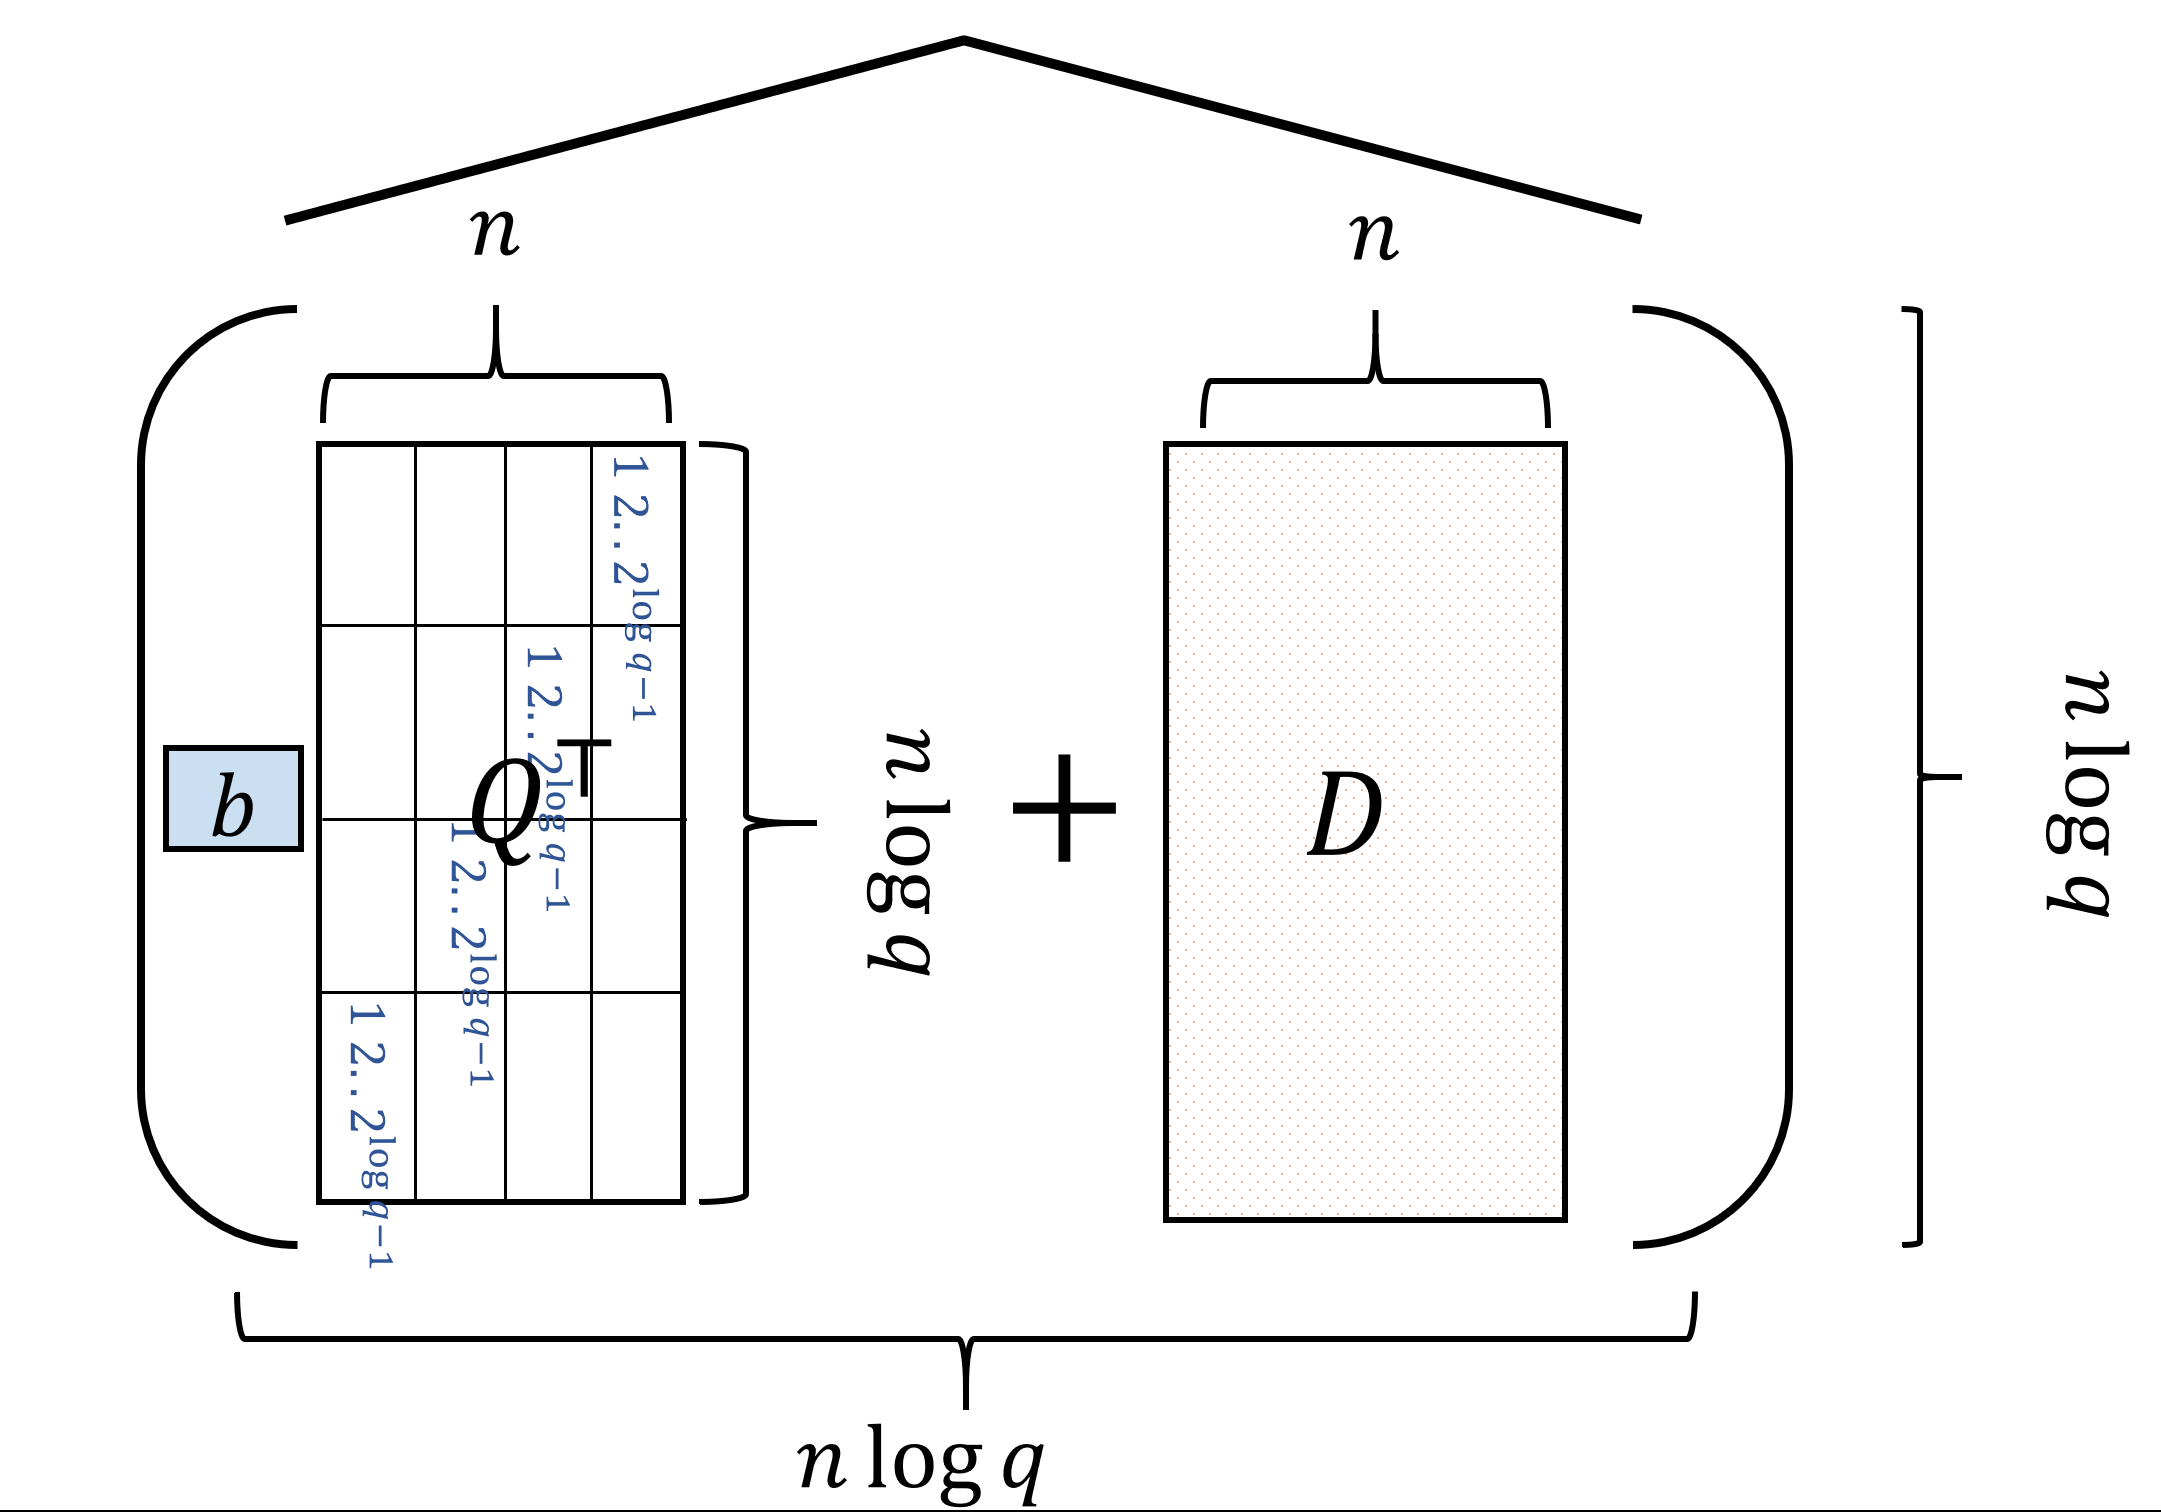
\includegraphics[width=\linewidth, height=1.5in, keepaspectratio]{../figure/fheenc.png}
\caption{In our fully homomorphic encryption, the public key is a
trapdoor generator \(G_s\). To encrypt a bit \(b\), we output
\(C=\widehat{(bQ^\top +D)}\) where \(D\) is a \((n\log q) \times n\)
matrix whose rows are generated using \(G_s\).}
\label{fheencfig}
\end{marginfigure}

\begin{marginfigure}
\centering
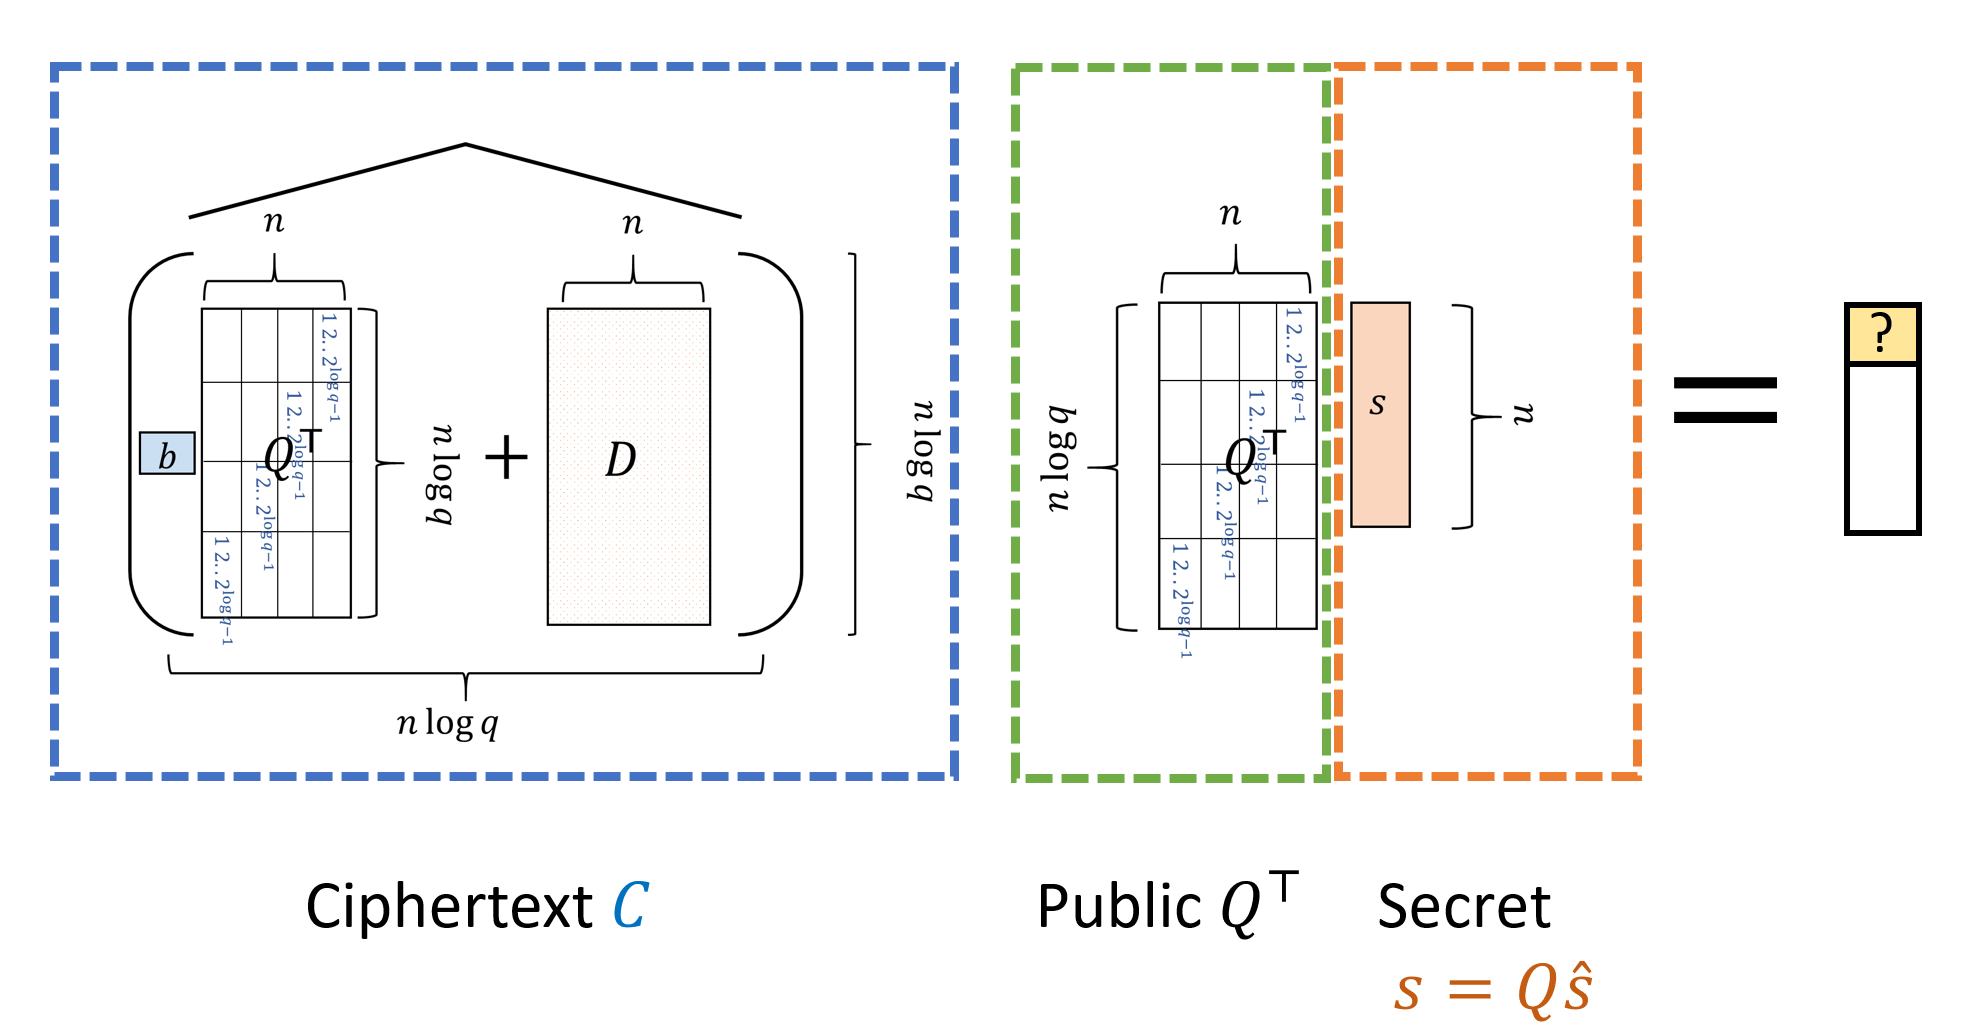
\includegraphics[width=\linewidth, height=1.5in, keepaspectratio]{../figure/fhedec.png}
\caption{We decrypt a ciphertext \(C=\widehat{(bQ^\top +D)}\) by looking
at the first coordinate of \(\ensuremath{\mathit{CQ}}^\top s\) (or
equivalently, \(\ensuremath{\mathit{CQ}}^\top Q\hat{s}\)). If \(b=0\)
then this equals to the first coordinate of \(Ds\), which is at most
\(\sqrt{q}\) in magintude. If \(b=1\) then we get an extra factor of
\(Q^\top s\) which we set to be in the interval \((0.499q,0.51q)\). We
can think of either \(s\) or \(\hat{s}\) as our secret key.}
\label{fhedecfig}
\end{marginfigure}

\section{Analysis of our scheme}\label{Analysis-of-our-scheme}

To show that that this scheme is a valid partially homomorphic scheme we
need to show the following properties:

\begin{enumerate}
\def\labelenumi{\arabic{enumi}.}
\item
  \textbf{Correctness:} The decryption of an encryption of
  \(b\in\{0,1\}\) equals \(b\).
\item
  \textbf{CPA security:} An encryption of \(0\) is computationally
  indistinguishable from an encryption of \(1\) to someone that got the
  public key.
\item
  \textbf{Homomorphism:} If \(C\) encrypts \(b\) and \(C'\) encrypts
  \(b'\) then \(C \overline{\wedge} C'\) encrypts
  \(b\; \ensuremath{\mathit{NAND}}\; b'\) (with a higher amount of
  noise). The growth of the noise will be the reason that we will not
  get immediately a fully homomorphic encryption.
\item
  \textbf{Shallow decryption circuit:} To plug this scheme into the
  bootstrapping theorem we will need to show that its decryption
  algorithm (or more accurately, the function in the statement of the
  bootstrapping theorem) can be evaluated in depth \(polylog(n)\)
  (independently of \(q\)), and that moreover, the noise grows slowly
  enough that our scheme is homomorphic with respect to such circuits.
\end{enumerate}

Once we obtain 1-4 above, we can plug FHEENC into the Bootstrapping
Theorem (\cref{bootstrapthm}) and thus complete the proof of existence
of a fully homomorphic encryption scheme. We now address those points
one by one.

\subsection{Correctness}\label{Correctness}

Correctness of the scheme will follow from the following stronger
condition:

\hypertarget{fhecorrectlem}{}
\begin{lemma} \label[lemma]{fhecorrectlem}

For every \(b \in \{0,1\}\), if \(C\) is the encryption of \(b\) then it
is an \((n\log q)\times (n \log q)\) matrix satisfying
\[\ensuremath{\mathit{CQ}}^\top s = bQ^\top s + e\] where
\(\max |e_i| \ll \sqrt{q}\).

\end{lemma}

\begin{proof} \label[proof]{For-starters-let-us-see-that-t}

For starters, let us see that the dimensions make sense: the encryption
of \(b\) is computed by \(C=\widehat{(bQ^\top +D)}\) where \(D\) is an
\((n\log q)\times n\) matrix satisfying \(|Ds|_i \leq \sqrt{q}\) for
every \(i\).

Since \(Q^\top\) is also an \((n \log q) \times n\) matrix, adding
\(bQ^\top\) (i.e.~either \(Q^\top\) or the all-zeroes matrix, depending
on whether or not \(b=1\)) to \(D\) makes sense and applying the
\(\hat{\cdot}\) operation will transform every row to length \(n\log q\)
and hence \(C\) is indeed a square \((n\log q)\times (n \log q)\)
matrix.

Let us now see what this matrix \(C\) does to the vector \(v=Q^\top s\).
Using the fact that \(\hat{M}Q^\top = M\) for every matrix \(M\), we get
that \[Cv = (bQ^\top + D) s = bv+  Ds\] but by construction
\(|(Ds)_i| \leq \sqrt{q}\) for every \(i\).

\end{proof}

\cref{fhecorrectlem} implies correctness of decryption since by
construction we ensured that \((Q^\top s)_1 \in (0.499q,0.5001q)\) and
hence we get that if \(b=0\) then \(|(Cv)_1|=o(q)\) and if \(b=1\) then
\(0.499q-o(q) \leq |(C_v)_1| \leq 0.501q + o(q)\).

\subsection{CPA Security}\label{CPA-Security}

To show CPA security we need to show that an encryption of \(0\) is
indistinguishable from an encryption of \(1\). However, by the security
of the trapdoor generator, an encryption of \(b\) computed according to
our algorithm will be indistinguishable from an encryption of \(b\)
obtained when the matrix \(D\) is a random \((n\log q)\times n\) matrix.
Now in this case the encryption is obtained by applying the
\(\hat{\cdot}\) operation to \(bQ^\top +D\) but if \(D\) is uniformly
random then for every choice of \(b\), \(bQ^\top + D\) is uniformly
random (since a fixed matrix plus a random matrix yields a random
matrix) and hence the matrix \(bQ^\top + D\) (and so also the matrix
\(\widehat{bQ^\top+D}\)) contains no information about \(b\). This
completes the proof of CPA security (can you see why?).

If we want to plug in this scheme in the bootstrapping theorem, then we
will also assume that it is \emph{circular secure}. It seems a
reasonable assumption though unfortuantely at the moment we do not know
how to derive it from LWE. (If we don't want to make this assumption we
can still obtained a \emph{leveled} fully homomorphic encryption as
discussed in the previous lecture.)

\subsection{Homomorphism}\label{Homomorphism}

Let \(v=Qs\), \(b\in\{0,1\}\) and \(C\) be a ciphertext such that
\(Cv = bv + e\). We define the \emph{noise} of \(C\), denoted as
\(\mu(C)\) to be the maximum of \(|e_i|\) over all \(i\in[n\log q]\). We
make the following lemma, which we'll call the ``noisy homomorphism
lemma'':

\hypertarget{noisehomolem}{}
\begin{lemma} \label[lemma]{noisehomolem}

Let \(C,C'\) be ciphertexts encrypting \(b,b'\) respectively with
\(\mu(C),\mu(C')\leq q/4\). Then \(C''=C \overline{\wedge} C'\) encrypts
\(b\; \ensuremath{\mathit{NAND}}\; b'\) and satisfies
\[\mu(C'') \leq (2n\log q)\max\{ \mu(C), \mu(C') \} \label{eqnoisebound}\]

\end{lemma}

\begin{proof} \label[proof]{This-follows-from-the-calculat}

This follows from the calculations we have done before. As we've seen,
\[\widehat{CQ^\top}C'v = \widehat{CQ^\top}(b'v+e') = b'\widehat{CQ^\top}Q^\top s + \widehat{CQ^\top}e' = b'(Cv)+ \widehat{CQ^\top}e' = bb'v + b'e+ \widehat{CQ^\top}e'\]
But since \(\widehat{CQ^\top}\) is a \(0/1\) matrix with every row of
length \(n\log q\), for every \(i\)
\((\widehat{CQ^\top}e')_i \leq (n\log q)\max_j |e_j|\). We see that the
noise vector in the product has magnitude at most
\(\mu(C)+n\log q \mu(C')\). Adding the identity for the NAND operation
adds at most \(\mu(C)+\mu(C')\) to the noise, and so the total noise
magnitude is bounded by the righthand side of \eqref{eqnoisebound}.

\end{proof}

\subsection{Shallow decryption
circuit}\label{Shallow-decryption-circuit}

Recall that to plug in our homomorphic encryption scheme into the
bootstrapping theorem, we needed to show that for every ciphertexts
\(C,C'\) (generated by the encryption algorithm) the function
\(f:\{0,1\}^{n \log q} \rightarrow \{0,1\}\) defined as
\[f(d) = D_d(C) \;\ensuremath{\mathit{NAND}}\; D_d(C')\] can be
homomorphically evaluated where \(d\) is the secret key and \(D_d(C)\)
denotes the decryption algorithm applied to \(C\).

In our case we can think of the secret key as the binary string
\(\hat{s}\) which describes our vector \(s\) as a bit string of length
\(n\log q\). Given a ciphertext \(C\), the decryption algorithm takes
the dot product modulo \(q\) of \(s\) with the first row of
\(\ensuremath{\mathit{CQ}}^\top\) (or, equivalently, the dot product of
\(\hat{s}\) with the first row of \(\ensuremath{\mathit{CQ}}^\top Q\))
and outputs \(0\) (respectively \(1\)) if the resulting number is small
(respectively large).

By repeatedly applying the noisy homomorphism lemma
(\cref{noisehomolem}), we can show that can homorphically evaluate every
circuit of NAND gates whose \emph{depth} \(\ell\) satisfies
\((2n\log q)^\ell \ll q\). If \(q = 2^{\sqrt{n}}\) then (assuming \(n\)
is sufficiently large) then as long as \(\ell < n^{0.49}\) this will be
satisfied.

In particular to show that \(f(\cdot)\) can be homomorphically evaluated
it will suffice to show that for every fixed vector
\(c\in \Z_q^{n\log q}\) there is a \(polylog(n) \ll n^{0.49}\) depth
circuit \(F\) that on input a string \(\hat{s}\in\{0,1\}^{n \log q}\)
will output \(0\) if \(|\langle c,\hat{s \rangle}| < q/10\) and output
\(1\) if \(|\langle c,\hat{s \rangle}| > q/5\). (We don't care what
\(F\) does otherwise. The above suffices since given a ciphertext \(C\)
we can use \(F\) with the vector \(c\) being the top row of
\(\ensuremath{\mathit{CQ}}^\top Q\), and hence
\(\langle c,\hat{s} \rangle\) would correspond to the first entry of
\(\ensuremath{\mathit{CQ}}^\top s\). Note that if \(F\) has depth
\(\ell\) then the function \(f()\) above has depth at most \(\ell+1\).)

\begin{pause} \label[pause]{Please-make-sure-you-understan}

Please make sure you understand the above argument.

\end{pause}

If \(c=(c_1,\ldots,c_{n\log q})\) is a vector then to compute its inner
product with a \(0/1\) vector \(\hat{s}\) we simply need to sum up the
numbers \(c_i\) where \(\hat{s}_i=1\). Summing up \(m\) numbers can be
done via the obvious recursion in depth that is \(\log m\) times the
depth for a single addition of two numbers. However, the naive way to
add two numbers in \(\Z_q\) (each represented by \(\log q\) bits) will
have depth \(O(\log q)\) which is too much for us.

\begin{pause} \label[pause]{Please-stop-here-and-see-if-yo}

Please stop here and see if you understand why the natural circuit to
compute the addition of two numbers modulo \(q\) (represented as
\(\log q\)-length binary strings) will require depth \(O(\log q)\). As a
hint, one needs to keep track of the ``carry''.

\end{pause}

Fortunately, because we only care about accuracy up to \(q/10\), if we
add \(m\) numbers, we can drop all but the first \(100\log m\) most
significant digits of our numbers, since including them can change the
sum of the \(m\) numbers by at most \(m(q/m^{100}) \ll q\). Hence we can
easily do this work in \(poly(\log m)\) depth, which is \(poly(\log n)\)
since \(m=poly(n)\).

Let us now show this more formally:

\hypertarget{decdepthlem}{}
\begin{lemma} \label[lemma]{decdepthlem}

For every \(c\in\Z_q^m\) there exists some function
\(f:\{0,1\}^m\rightarrow\{0,1\}\) such that:\\
1. For every \(\hat{s}\in \{0,1\}^n\) such that
\(|\langle \hat{s} \rangle,c|<0.1q\), \(f(\hat{s})=0\)\\
2. For every \(\hat{s}\in \{0,1\}^n\) such that
\(0.4q<|\langle \hat{s} \rangle,c|<0.6q\), \(f(\hat{s})=1\)\\
3. There is a circuit computing \(f\) of depth at most
\(100(\log m)^3\).

\end{lemma}

\begin{proof} \label[proof]{For-every-number-xinZq-write-t}

For every number \(x\in\Z_q\), write \(\tilde{x}\) to be the number that
is obtained by writing \(x\) in the binary basis and setting all digits
except the \(10\log m\) most significant ones to zero.\\
Note that \(\tilde{x} \leq x \leq \tilde{x} + q/m^{10}\). We define
\(f(\hat{s})\) to equal \(1\) if
\(|\sum \hat{s}_i \tilde{c}_i (\mod \tilde{q})| \geq 0.3\tilde{q}\) and
to equal \(0\) otherwise (where as usual the absolute value of \(x\)
modulo \(\tilde{q}\) is the minimum of \(x\) and \(\tilde{q}-x\).) Note
that all numbers involved have zeroes in all but the \(10\log m\) most
significant digits and so these less significant digits can be ignored.
Hence we can add any pair of such numbers modulo \(\tilde{q}\) in depth
\(O(\log m)^2\) using the standard elementary school algorithm to add
two \(\ell\)-digit numbers in \(O(\ell^2)\) steps. Now we can add the
\(m\) numbers by adding pairs, and then adding up the results, and this
way in a binary tree of depth \(\log m\) to get a total depth of
\(O(\log m)^3\). So, all that is left to prove is that this function
\(f\) satisfies the conditions (1) and (2).

Note that
\(|\sum \hat{s}_i \tilde{c}_i - \sum \hat{s}_i c_i | < mq/m^{10} = q/m^9\)
so now we want to show that the effect of taking modulo \(\tilde{q}\) is
not much different from taking modulo \(q\). Indeed, note that this sum
(before a modular reduction) is an integer between \(0\) and \(qm\). If
\(x\) is such an integer and we divide \(x\) by \(q\) to write
\(x = kq+ r\) for \(r<q\), then since \(x<qm\), \(k<m\), and so we can
write \(x = k\tilde{q} + k(q-\tilde{q})+r\) so the difference between
\(k \mod q\) and \(k \mod{\tilde{q}}\) will be (in our standard modular
metric) at most \(mq/m^{10}=q/m^9\). Overall we get that if
\(\sum \hat{s}_i c_i \mod{q}\) is in the interval \([0.4q, 0.6q]\) then
\(\sum \hat{s}_i \tilde{c}_i ( \mod{\tilde{q}})\) will be in the
interval \([0.4q-100q/m^9, 0.6q+100q/m^9]\) which is contained in
\([0.3\tilde{q},0.7\tilde{q}]\).

\end{proof}

This completes the proof that our scheme can fit into the bootstrapping
theorem (i.e., of \cref{LWEFHEthm}), hence completing the description of
the fully homomorphic encryption scheme.

\begin{pause} \label[pause]{Now-would-be-a-good-point-to-g}

Now would be a good point to go back and see you understand how all the
pieces fit together to obtain the complete construction of the fully
homomorphic encryption scheme.

\end{pause}

\section{Advanced topics:}\label{Advanced-topics}

\subsection{Fully homomorphic encryption for approximate computation
over the real numbers:
\href{https://eprint.iacr.org/2016/421.pdf}{CKKS}}\label{Fully-homomorphic-encryption-f}

We have seen how a fully homomorphic encryption for a plaintext bit
\(b\) can be constructed and we are able to evaluate addition and
multiplication of ciphertexts as well as a NAND gate in the ciphertext
space. One can also extend FHEENC scheme to encrypt a plaintext message
\(\mu \in \Z_q\) and can evaluate multi-bit integer additions and
multiplications more efficiently. Our next following question would be
floating/fixed point operations. They are similar to integer operations,
but we need to be able to evaluate a rounding operation following every
computation. Unfortunately, it has been considered difficult to evaluate
the rounding operation ensuring the correctness property. An easier
solution is to assume approximate computations from the beginning and
embrace errors caused by them.

CKKS scheme, one of the recent schemes, addressed this challenge by
allowing small errors in the decrypted results. Its correctness property
is more relaxed than what we've seen before. Now decryption does not
necessarily be precisely the original message, and indeed, this resolved
the rounding operation problem supporting approximate computation over
the real numbers. To get more sense on its construction, recall that
when we decrypt a ciphertext in the FHEENC scheme, we have
\(\ensuremath{\mathit{CQ}}^\top s = bQ^\top s + e\) where
\(\max |e_i| \ll \sqrt{q}\). Since
\((Q^\top s)_1 \in (0.499q, 0.5001q)\), multiplying by this term places
a plaintext bit near the most significant bits of the ciphertext where
the plaintext cannot be polluted by the encryption noise. Therefore, we
are able to precisely remove the noise \(e\) we added for the security.
However, this kind of separated placement actually makes an evaluation
of the rounding operation difficult. On the other hand, the CKKS scheme
doesn't clearly separate the plaintext message and noise in its
decryption structure. Specifically, we have the form of
\(c^\top s = m + e\) and the noise lies with the LSB part of the message
and does pollute the lowest bits of the message. Note that this is
acceptable as long as it preserves enough precision. Now we can evaluate
rounding(i.e., rescaling in the paper) homomorphically, by dividing both
a ciphertext \(c\) and the parameter \(q\) by some factor \(p\). The
concept of handling ciphertexts with a different encryption parameter
\(q'=q/p\) is already known to be possible. You can find more details on
this modulus switching technique in this
\href{https://eprint.iacr.org/2011/277.pdf}{paper} if you are
interested. Besides, it is also proved that the precision loss of the
decrypted evaluation result is at most one more bit loss compared to the
plaintext computation result, which means the scheme's precision
guarantee is nearly optimal. This scheme offers an efficient homomorphic
encryption setting for many practical data science and machine learning
applications which does not require precise values, but approximate
ones. You may check existing open source libraries, such as
\href{https://www.microsoft.com/en-us/research/project/microsoft-seal/}{MS
SEAL} and \href{https://github.com/snucrypto/HEAAN}{HEAAN}, of this
scheme as well as many practical applications including
\href{https://eprint.iacr.org/2018/254.pdf}{logistic regression} in the
literature.

\subsection{Bandwidth efficient fully homomorphic encryption
\href{https://eprint.iacr.org/2019/733.pdf}{GH}}\label{Bandwidth-efficient-fully-homo}

When we define homomorphic encryption in \cref{partialhomdef}, we only
consider a class of single-output functions \(\mathcal{F}\). Now we want
to extend the difinition to multiple-output function and consider how
bandwidth-efficient the fully homomorphic encryption can be. More
specifically, if we want to guarantee that the result of decryption is
(or contains) \(f(x_1,\ldots,x_\ell)\), what will be the minimal
possible length of the ciphertext? Let us first define the compressible
fully homomorphic encryption scheme.

::: \{.definition title=``Compressible Fully Homomorphic Encryption''
\#compFHE\} A \emph{compressible fully homomorphic public key encryption
scheme} is a CPA secure public key encryption scheme \((G,E,D)\) such
that there exist polynomial-time algorithms
\(\ensuremath{\mathit{EVAL}}, \ensuremath{\mathit{COMP}}:{0,1}^* \rightarrow {0,1}^*\)
such that for every \((e,d)=G(1^n)\), \(\ell=poly(n)\),
\(x_1,\ldots,x_\ell \in \{0,1\}\), and
\(f:\{0,1\}^\ell\rightarrow \{0,1\}^*\) which can be described by a
circuit, it holds that:

\begin{itemize}
\item
  \(c=\ensuremath{\mathit{EVAL}}_e(f,E_e(x_1),\ldots,E_e(x_\ell))\).
\item
  \(c^*=\ensuremath{\mathit{COMP}}(c)\).
\item
  \(f(x_1,\ldots,x_\ell)\) is a prefix of \$D\_d(c\^{}*) \$. :::
\end{itemize}

This definition is similar to the standard fully homomorphic encryption
except an additional compression step. The bandwidth efficiency of a
compressible fully homomorphic encryption is often described by the rate
which is defined as follows:

::: \{.definition title=``Rate of Compressible Fully Homomorphic
Encryption'' \#ratecompFHE\} A compressible fully homomorphic public key
encryption scheme has \emph{rate} \(\alpha=\alpha(n)\) if for every
\((e,d)=G(1^n)\), \(\ell=poly(n)\), \(x_1,\ldots,x_\ell \in \{0,1\}\),
and \(f:\{0,1\}^\ell\rightarrow \{0,1\}^*\) with sufficiently long
output, it holds that \[\alpha |c^*|\leq |f(x_1,\ldots,x_\ell)|.\] :::

The following theorem answers the earlier question, which states that
the nearly optimal rate, say a rate arbitrarily close to 1, can be
achieved.

\hypertarget{optrate}{}
\begin{theorem}[Nearly Optimal Rate, [Gentry and Halevi 2019](https://eprint.iacr.org/2019/733.pdf)] \label[theorem]{optrate}

For any \(\epsilon>0\), there exists a compressive fully homomorphic
encryption scheme with rate being \(1-\epsilon\) under the LWE
assumption.

\end{theorem}

\subsection{Using fully homomorphic encryption to achieve private
information retrieval.}\label{Using-fully-homomorphic-encryp}

Private information retrieval (PIR) allows the client to retrive the
\(i\)-th entry of a database which has totally \(n\) entries without
letting the server know \(i\). We only consider the single-server case
here. Obviously, a trivial solution is that the server sends the entire
database to the client.

One simple case of PIR is that each entry is a bit, for which the
trivial solution above has the communication complexity being \(n\).
\href{https://web.cs.ucla.edu/~rafail/PUBLIC/34.pdf}{Kushilevitz and
Ostrovsky 1997} reduced the the complexity to be smaller than
\(O(n^\epsilon)\) for any \(\epsilon>0\). After that, another work
(\href{https://people.csail.mit.edu/silvio/Selected\%20Scientific\%20Papers/Private\%20Information\%20Retrieval/Computationally\%20Private\%20Information\%20Retrieval\%20with\%20Polylogarithmic\%20Communication.pdf}{Cachin
et al.~1999}) further reduced the complexity to \(polylog(n)\). More
discussion about PIR and related FHE techniques can be found in
\href{https://eprint.iacr.org/2007/059.pdf}{Ostrovsky and Skeith 2007},
\href{https://ieeexplore.ieee.org/document/6189348}{Yi et al.~2013} and
references therein.

One interesting observation is that fully homomorphic encryption can be
applied to the single-server PIR via the following procedures:

\begin{itemize}
\item
  The client computes \(E_e(i)\) and sends it to the server.
\item
  The server evaluates \(c=\ensuremath{\mathit{EVAL}}(f,E_e(i))\), where
  \(f(i)\) returns the \(i\)-th entry of the database, and sends it (or
  its compressed version \(c^*\)) back to the client.
\item
  The client decrypts \(D_d(c)\) or \(D_d(c^*)\) and obtains the
  \(i\)-th entry of the database.
\item
  Bandwidth efficient fully homomorphic encryption
  \href{https://eprint.iacr.org/2019/733.pdf}{GH}
\end{itemize}

Since there exists compressive fully homomorphic encryption scheme with
nearly optimal rate, say rate arbitrary close to \(1\) (see
\cref{optrate}), we can immediately get rate-\((1-\epsilon)\) PIR for
any \(\epsilon\). (Note that this result holds only for database whose
entries is quite large, since the rate is defined for circuits with
sufficiently long output.) Prior to the theorem by
\href{https://eprint.iacr.org/2019/733.pdf}{Gentry and Halevi 2019},
\href{https://petsymposium.org/2015/papers/23_Kiayias.pdf}{Kiayias et
al.~2015} also constructed a PIR scheme with a nearly optimal
rate/bandwidth efficiency. The application of fully homomorphic
encryption to PIR is a fascinating field; not only limited to the
bandwidth efficiency, you may be also interested in the computational
cost. We refer to \href{https://eprint.iacr.org/2019/733.pdf}{Gentry and
Halevi 2019} for more details.
